\documentclass[serif]{beamer}

% default page size is:
% \beamer@paperwidth 12.80cm%
% \beamer@paperheight 9.60cm%

\setbeamersize{text margin left=0.4cm,text margin right=0.4cm}

\usepackage{tikz}
\usetikzlibrary{positioning,decorations.pathreplacing}

\usepackage{algorithm}
\usepackage[noend]{algpseudocode}

% symbols
\usepackage{amsmath} % assumes amsmath package installed
\usepackage{amssymb} % for \square
% non-italicized math subscripts
\newcommand{\ms}[1]{\mbox{\scriptsize #1}}
% from http://tex.stackexchange.com/a/5255
\DeclareMathOperator*{\argmin}{arg\,min}

% fonts
\renewcommand\rmdefault{pplx}
\renewcommand\mathfamilydefault{cmr}

\setbeamertemplate{navigation symbols}{}

\setbeamerfont{page number in head/foot}{size=\large}
%\setbeamertemplate{footline}[frame number]
\setbeamertemplate{footline}{%
   \raisebox{7pt}{\makebox[\paperwidth]{%
   \hfill\makebox[10pt]{\textcolor{gray}{%
   \large\insertframenumber\hspace{0.1in}}}}}}

% dont number title page
\addtocounter{framenumber}{-1}

\title{Efficient Manipulation Task Planning via
Reuse-Informed Optimization of Planning Effort}
\author{Christopher M. Dellin}
\date{April 7, 2015}

\begin{document}

% HOW DOES IT FAIL?

\begin{frame}[plain]
   %\begin{columns}
   %   \column{1.2\textwidth}
      \maketitle
   %\end{columns}
\end{frame}

% first frame:
% REAL ROBOTS! REAL-WORLD PROBLEMS!
% overview of manipulation planning problem?
\begin{frame}

\the\textwidth

%\frametitle{First Slide}

   \begin{columns}
   \begin{column}{0.33\textwidth}
   \begin{center}
      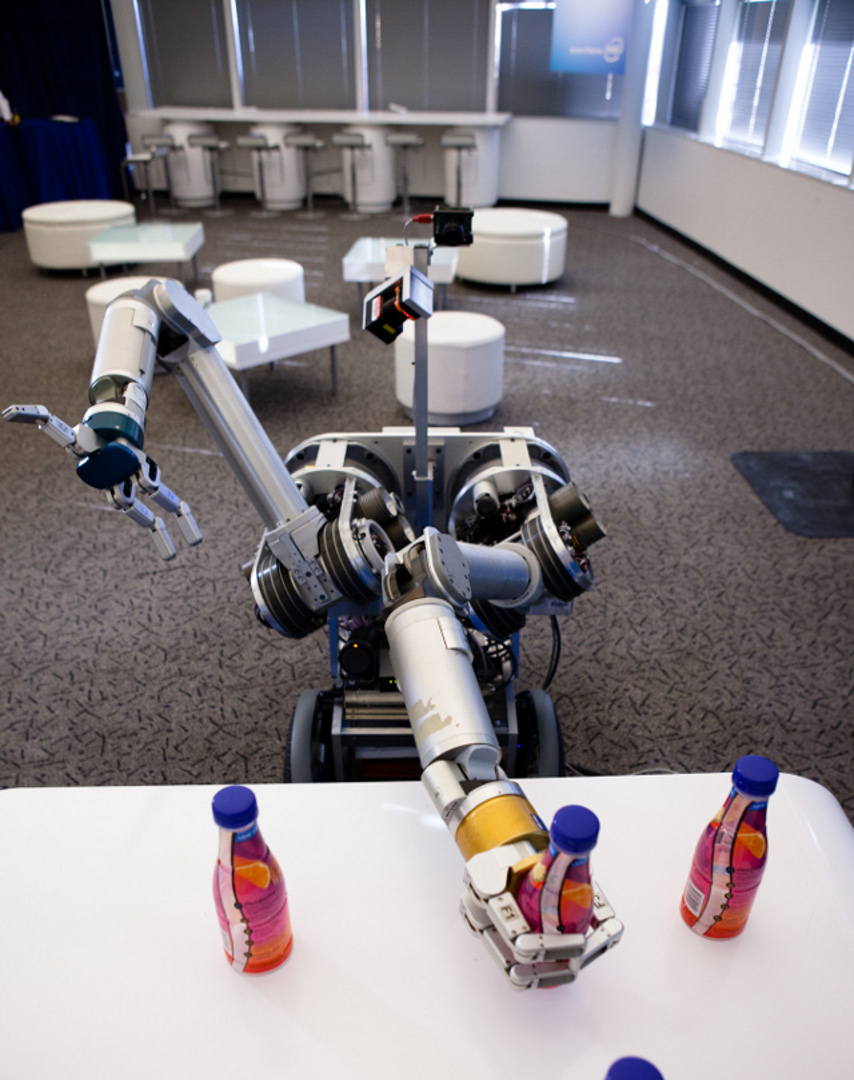
\includegraphics[width=\columnwidth]{images/herb.jpg}
      
      Herb
   \end{center}
   \end{column}%
   \begin{column}{0.33\textwidth}
   \begin{center}
      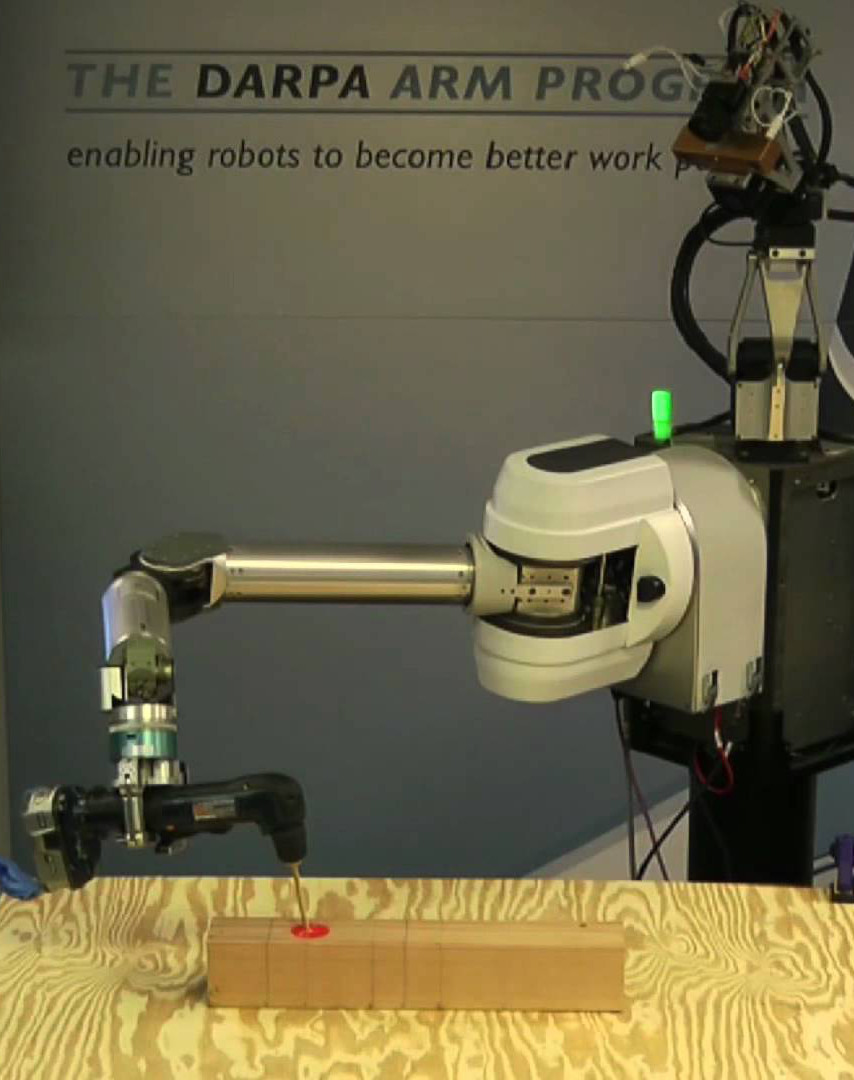
\includegraphics[width=\columnwidth]{images/arms.jpg}
      
      ARM-S
   \end{center}
   \end{column}%
   \begin{column}{0.33\textwidth}
   \begin{center}
      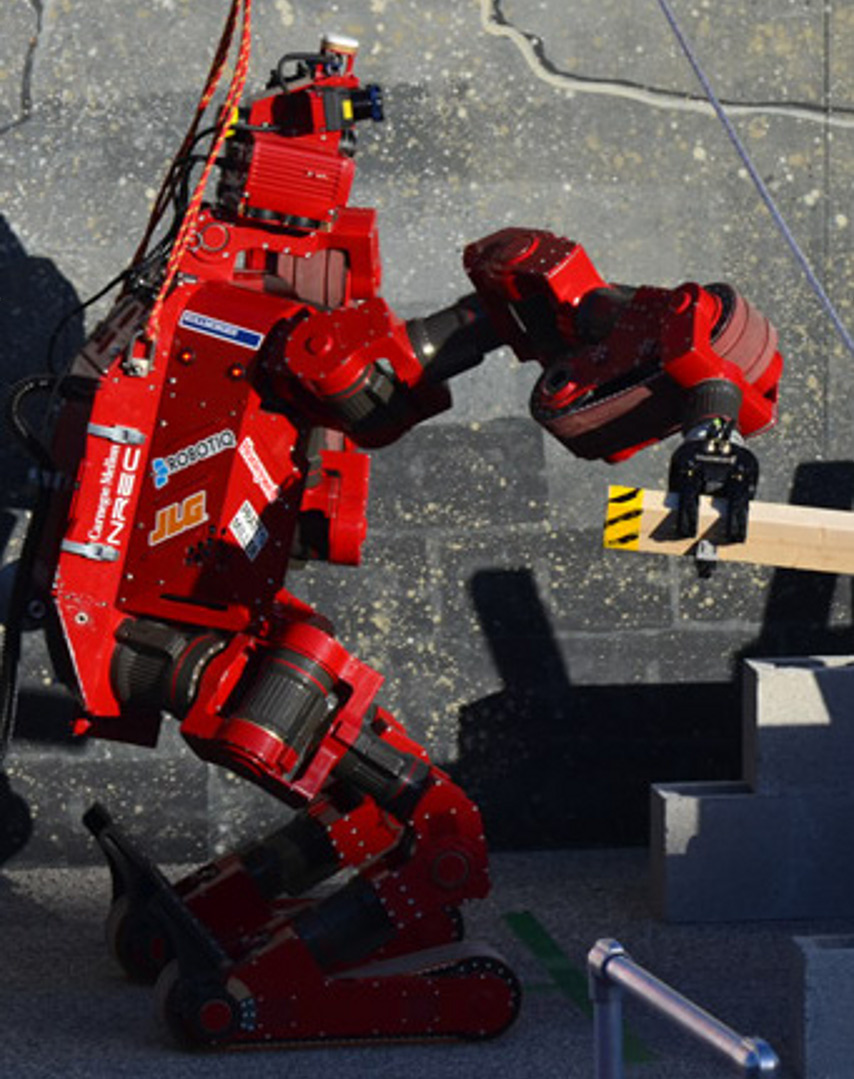
\includegraphics[width=\columnwidth]{images/chimp.jpg}
      
      Chimp
   \end{center}
   \end{column}
   \end{columns}

   General description of manipulation tasks.

   (a) Unpredictable world with lots of objects,
   (b) sensors that build a geometric model,
   (c) planning motion with onboard computation,
   (d) executing motion using articulated arms.

   (Takeaway: {\bf Real-world} manipulation tasks.)

\end{frame}

\begin{frame}
   Video collage of these robots (plus PR-2?) performing manipulation tasks.

   Call out {\bf 10x} in the corner of each screen.
   Joke opportunity.

   Takeaway: total task time is too slow.
   {\bf Why is that?}
\end{frame}

%\begin{frame}
%   \frametitle{tasks are slow because planning is slow}
%   
%   Make figure:
%   \begin{tabular}{ll}
%      HERB pic & 50\% planning time, 50\% exec time \\
%      CHIMP pic & 40\% planning time, 60\% exec time \\
%   \end{tabular}
%   
%   \medskip
%   Focus on planning for manipulation tasks.
%   Talk about WHY planning is slow, and WHY planning is necesary
%   in these problems.
%   
%   \medskip
%   Do I need this slide?
%\end{frame}

\begin{frame}
   \frametitle{Example problem, and scope}

   \begin{center}
      VIDEO:
      
      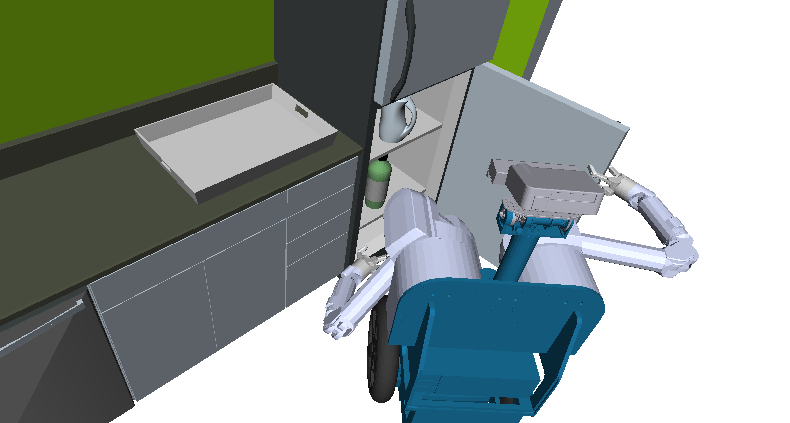
\includegraphics[width=\textwidth]{figs/fridge-intro.png}
      
      %\includegraphics[width=0.8\textwidth]{build/diagram-mutlistep-intro}
   \end{center}
   
   In order to describe why it's so slow,
   I need to talk a bit about the problem's structure
   and current approaches to handling it.
   
   To illustrated the challenges,
   here, look at this HERB example.
   
   (Below, show a 2d example of the multi-step problem.)

\end{frame}

%\begin{frame}
%   \frametitle{Structure of multi-step manipulation}
%   
%   INSERT IMAGE OF TASK
%   
%   \begin{center}
%   
%      %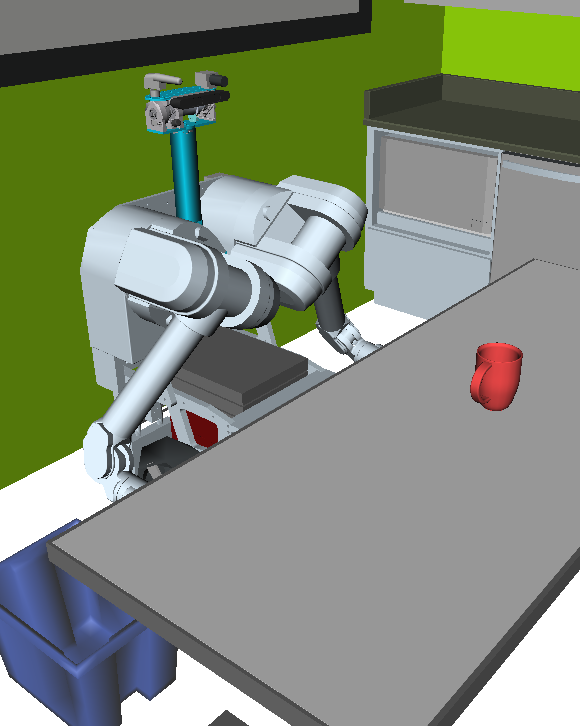
\includegraphics[width=0.19\linewidth]{figs/testherb-a.png}
%      %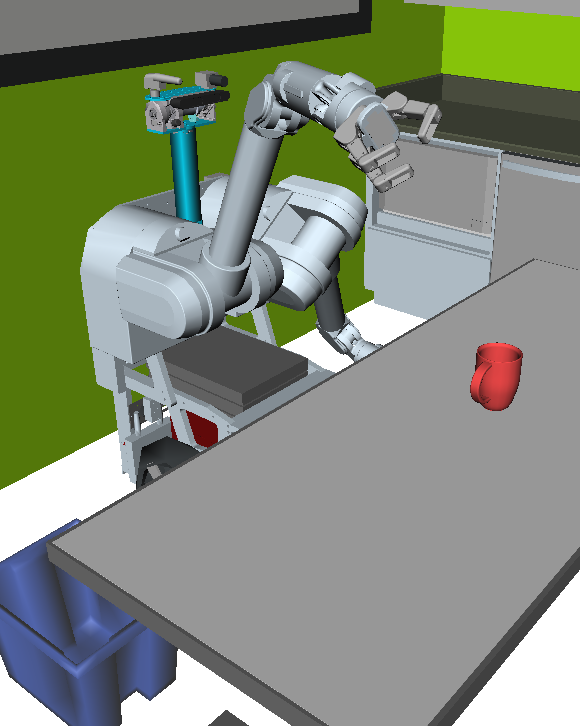
\includegraphics[width=0.19\linewidth]{figs/testherb-b.png}
%      %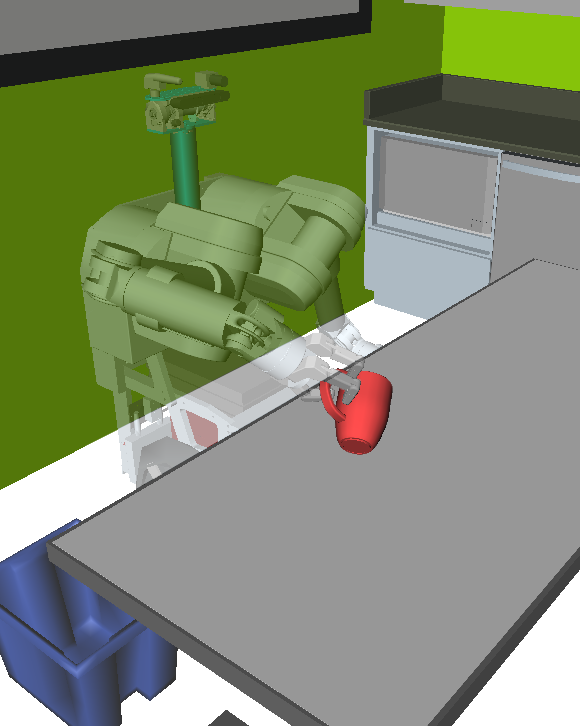
\includegraphics[width=0.19\linewidth]{figs/testherb-c.png}
%      %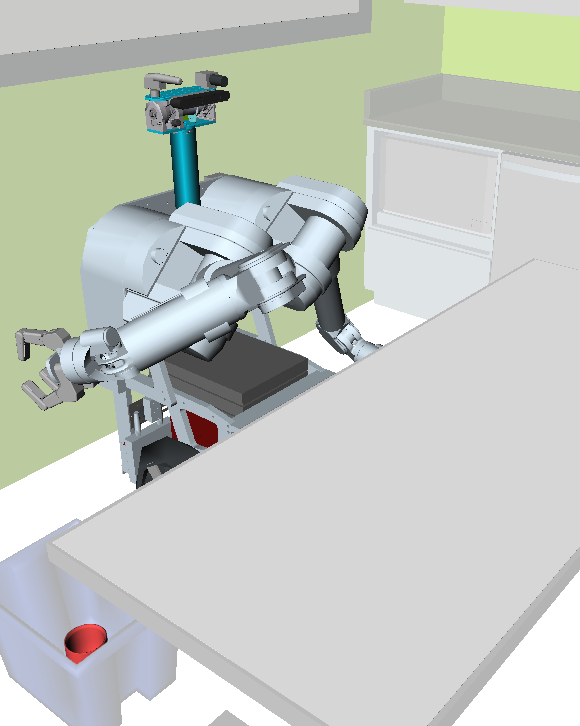
\includegraphics[width=0.19\linewidth]{figs/testherb-d.png}
%      %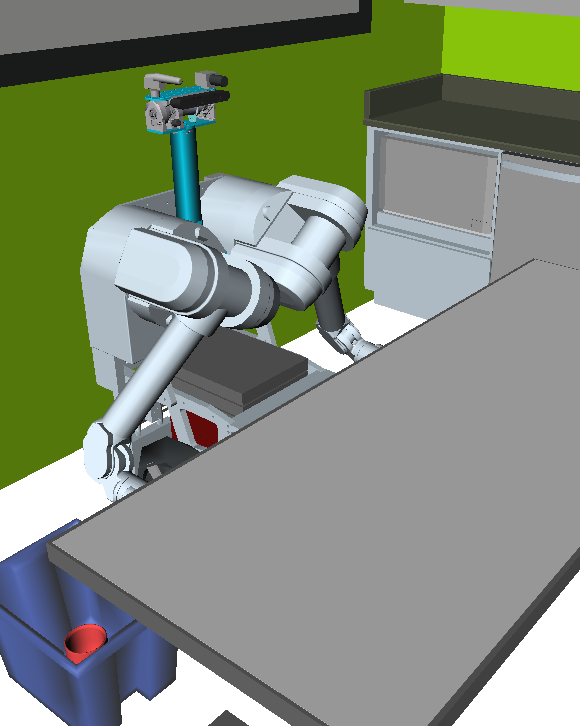
\includegraphics[width=0.19\linewidth]{figs/testherb-e.png}
%      
%      \includegraphics[width=2.5in]{build/diagram-multi-step}
%
%   \end{center}
%   
%   Overview.
%   
%   Challenge 1 is within steps.
%   
%   Challenge 2 is between steps.
%   
%   Challenge 3 is all steps taken together.
%\end{frame}

\begin{frame}
   \frametitle{Challenge 1: The Planning vs. Execution Tradeoff}

   \begin{center}
      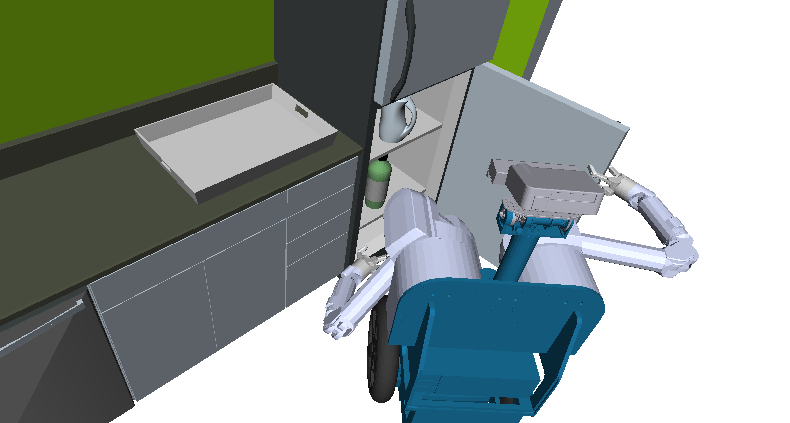
\includegraphics[width=0.6\textwidth]{figs/fridge-intro.png}
   \end{center}

   {\bf Minimize total task effort.}
   Planning effort is just as important as execution effort.
   
   \medskip

   Planning is expensive.
   Complex geometric models, many degrees of freedom.

   \medskip
   
   \includegraphics[width=0.3\textwidth]{build/talk-challenge1-tradeoff}
   
\end{frame}

\begin{frame}
   \frametitle{Challenge 2: Incongruent Steps Impede Reuse}

   Can we just cache everything?
   
   Typically, we do exploration in the robot's C-space.
   Each step is different.

   Every time you grab or release something,
   or something in the environment moves,
   which is all the time.
   
   \medskip
   \includegraphics[width=0.3\textwidth]{build/talk-challenge1-tradeoff}
   \includegraphics[width=0.3\textwidth]{build/talk-challenge1-tradeoff}
   
\end{frame}

\begin{frame}
   \frametitle{Challenge 3: Coupled Steps Require More Planning}

   Must plan several steps ahead to keep from getting stuck.
   
   Related to HPN?
   
   DRC kept getting stuck.
   
   \medskip
   \includegraphics[width=0.3\textwidth]{build/talk-challenge1-tradeoff}
   \includegraphics[width=0.3\textwidth]{build/talk-challenge1-tradeoff}
   \includegraphics[width=0.3\textwidth]{build/talk-challenge1-tradeoff}
   
\end{frame}

\begin{frame}
   \frametitle{Outline / Approach / Proposal Objective}
   
   Planning for manipulation tasks pose three challenges:
   
   \begin{itemize}
   \item Challenge 1: Planning each step is expensive.
   \item Challenge 2: Incongruent steps impede reuse.
   \item Challenge 3: Coupled steps make you get stuck or plan ahead.
   \end{itemize}
   
   The proposed work is a framework to address planning for
   manipulation tasks \emph{efficiently}.
   
\end{frame}

\begin{frame}
   \frametitle{Act 1: Capturing the Planning/Execution Tradeoff}
   
   \includegraphics[width=0.3\textwidth]{build/talk-challenge1-tradeoff}
   
   add P vs E PLOT
   
   add PREMISE: planning effort DOMINATED by configuration valitiy checking!s
\end{frame}
   
\begin{frame}
   \frametitle{Motion Planning in Configuration Space}
   \begin{tikzpicture}
   
      \draw[step=1,black!10,very thin] (0,0) grid (12,8);
      
      \node[inner sep=0] at (3,4)
         {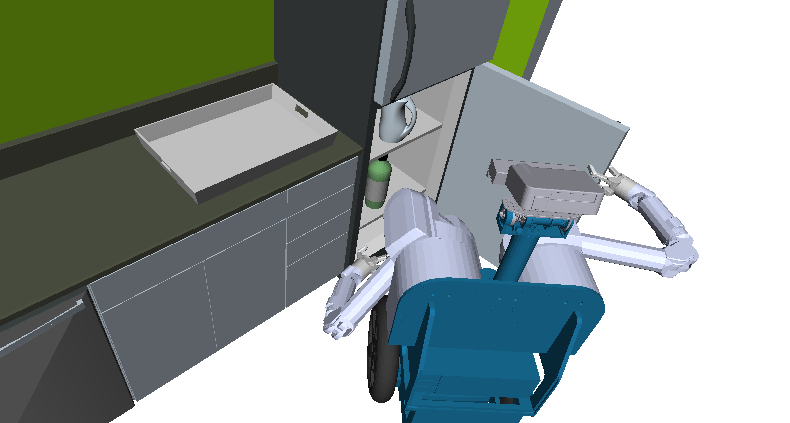
\includegraphics[width=5cm]{figs/fridge-intro.png}};
   
      \node[inner sep=0] at (9,5) {%
         {\only<1>{\includegraphics{build/talk-act1-2d}}}%
         {\only<2>{\includegraphics{build/talk-act1-2d,cfree}}}%
         {\only<3>{\includegraphics{build/talk-act1-2d,paths}}}%
      };
      
      % legend
      \only<2->{
         \node[draw,line width=1.5pt,fill=blue!20,minimum width=0.75cm,minimum height=0.10cm]
            (Cfreebox) at (3.0, 7.0) {};
         \node[right=0cm of Cfreebox] {: $\mathcal{C}_{\mbox{\scriptsize free}}$}; 
      }
      \only<3->{
         \node at (3,6.25) {$\Pi$ : set of candidate paths};
      }
      
      \only<1>{\node at (6,1) {High-dimensional C-space (cite TLP).};}
      \only<2>{\node at (6,1.3) {\begin{minipage}{11cm}\begin{center}
         \begin{equation*}
            f_x(\pi) = x(\pi)
         \end{equation*}
         Lots of possible paths.

         {\bf How to find low-cost paths quickly?}%
         \end{center}\end{minipage}
      };}
      \only<3>{\node at (6,1.3) {\begin{minipage}{11cm}\begin{center}
         \begin{equation*}
            f_x(\pi) =
            \left\{ \begin{array}{ll}
                x(\pi) & \mbox{if } {\bf 1}_{\mbox{\scriptsize free}}(\pi) \\
                \infty & \mbox{otherwise}
            \end{array} \right.
         \end{equation*}
         
         It has an indicator function,
         which is expensive to evaluate.
         \end{center}\end{minipage}
      };}
   
   \end{tikzpicture}
\end{frame}

\begin{frame}
   \frametitle{Best-First Search over Paths}
   \begin{tikzpicture}
   
      \draw[step=1,black!10,very thin] (0,0) grid (12,8);
      
      \node[inner sep=0] at (9,5) {%
         {\only<1>{\includegraphics{build/talk-act1-2d,paths}}}%
         {\only<2>{\includegraphics{build/talk-act1-2d,traja}}}%
         {\only<3>{\includegraphics{build/talk-act1-2d,firstfail}}}%
         {\only<4>{\includegraphics{build/talk-act1-2d,firstfailnext}}}%
      };
      
      % legend
      \node[draw,line width=1.5pt,fill=blue!20,minimum width=0.75cm,minimum height=0.10cm]
         (Cfreebox) at (3.0, 7.0) {};
      \node[right=0cm of Cfreebox] {: $\mathcal{C}_{\mbox{\scriptsize free}}$}; 
      \node at (3,6.25) {$\Pi$ : set of candidate paths};
      
      \only<1>{\fill[green!30] (0.5,4.1) rectangle (5.5,4.65);}
      \only<2>{\fill[green!30] (0.5,3.4) rectangle (5.5,4.1);}
      \only<3>{\fill[green!30] (0.5,2.9) rectangle (5.5,3.4);}
      \only<4>{\fill[green!30] (0.5,3.4) rectangle (5.5,4.65);}
      
      % bfs
      \node at (3,4) {\begin{minipage}{5cm}
         \begin{algorithmic}
         \Loop%
            \State $\Pi \leftarrow $ \textsc{GetPaths}$()$
            \State $\pi^* \leftarrow \argmin\limits_{\pi \in \Pi} f(\pi)$
            \State \textsc{EvalPath}$(\pi^*)$
         \EndLoop
         \end{algorithmic}
         \end{minipage}
      };
      
      \only<2>{\node at (6,1) {Select best candidate path.};}
      \only<3>{\node at (6,1) {Evaluate.};}
   
   \end{tikzpicture}
\end{frame}

\begin{frame}
   \frametitle{Best-First Search over Paths: RRTs}
   \begin{tikzpicture}
   
      \draw[step=1,black!10,very thin] (0,0) grid (12,8);
      
      \node[inner sep=0] at (9,5) {%
         {\only<1>{\includegraphics{build/talk-act1-2d,rrtstart}}}%
         {\only<2>{\includegraphics{build/talk-act1-2d,rrtsample}}}%
         {\only<3>{\includegraphics{build/talk-act1-2d,rrtcandidates}}}%
      };
      
      % legend
      \node[draw,line width=1.5pt,fill=blue!20,minimum width=0.75cm,minimum height=0.10cm]
         (Cfreebox) at (3.0, 7.0) {};
      \node[right=0cm of Cfreebox] {: $\mathcal{C}_{\mbox{\scriptsize free}}$}; 
      \node at (3,6.25) {$\Pi$ : set of candidate paths};
      
      \only<3>{\fill[green!30] (0.5,4.1) rectangle (5.5,4.65);}
      
      % bfs
      \node at (3,4) {\begin{minipage}{5cm}
         \begin{algorithmic}
         \Loop%
            \State $\Pi \leftarrow $ \textsc{GetPaths}$()$
            \State $\pi^* \leftarrow \argmin\limits_{\pi \in \Pi} f(\pi)$
            \State \textsc{EvalPath}$(\pi^*)$
         \EndLoop
         \end{algorithmic}
         \end{minipage}
      };
      
      %\only<2>{\node at (6,1) {Select best candidate path.};}
      %\only<3>{\node at (6,1) {Evaluate.};}
   
   \end{tikzpicture}
\end{frame}

\begin{frame}
   \frametitle{Best-First Search over Paths}
   \begin{tikzpicture}
   
      \draw[step=1,black!10,very thin] (0,0) grid (12,8);
      
      \node[inner sep=0] at (9,5) {%
         {\only<1>{\includegraphics{build/talk-act1-2d,firstfailnext}}}%
      };
      
      % legend
      \node[draw,line width=1.5pt,fill=blue!20,minimum width=0.75cm,minimum height=0.10cm]
         (Cfreebox) at (3.0, 7.0) {};
      \node[right=0cm of Cfreebox] {: $\mathcal{C}_{\mbox{\scriptsize free}}$}; 
      \node at (3,6.25) {$\Pi$ : set of candidate paths};
      
      \only<1>{\fill[green!30] (0.5,3.4) rectangle (5.5,4.65);}
      
      % bfs
      \node at (3,4) {\begin{minipage}{5cm}
         \begin{algorithmic}
         \Loop%
            \State $\Pi \leftarrow $ \textsc{GetPaths}$()$
            \State $\pi^* \leftarrow \argmin\limits_{\pi \in \Pi} f(\pi)$
            \State \textsc{EvalPath}$(\pi^*)$
         \EndLoop
         \end{algorithmic}
         \end{minipage}
      };
      
   \end{tikzpicture}
\end{frame}

\begin{frame}
   \frametitle{Best-First Search over Paths: Roadmaps}
   \begin{tikzpicture}
   
      \draw[step=1,black!10,very thin] (0,0) grid (12,8);
      
      \node[inner sep=0] at (9,5) {%
         {\only<1>{\includegraphics{build/talk-act1-2d,graph}}}%
         {\only<2>{\includegraphics{build/talk-act1-2d,graphfirst}}}%
         {\only<3>{\includegraphics{build/talk-act1-2d,graphfirstevaled}}}%
         {\only<4>{\includegraphics{build/talk-act1-2d,graphfirstnext}}}%
      };
      
      % legend
      \node[draw,line width=1.5pt,fill=blue!20,minimum width=0.75cm,minimum height=0.10cm]
         (Cfreebox) at (3.0, 7.0) {};
      \node[right=0cm of Cfreebox] {: $\mathcal{C}_{\mbox{\scriptsize free}}$}; 
      \node at (3,6.25) {$\Pi$ : set of candidate paths};
      
      \only<1>{\fill[green!30] (0.5,4.1) rectangle (5.5,4.65);}
      \only<2>{\fill[green!30] (0.5,3.4) rectangle (5.5,4.1);}
      \only<3>{\fill[green!30] (0.5,2.9) rectangle (5.5,3.4);}
      \only<4>{\fill[green!30] (0.5,3.4) rectangle (5.5,4.1);}
      
      % bfs
      \node at (3,4) {\begin{minipage}{5cm}
         \begin{algorithmic}
         \Loop%
            \State $\Pi \leftarrow $ \textsc{GetPaths}$()$
            \State $\pi^* \leftarrow \argmin\limits_{\pi \in \Pi} f(\pi)$
            \State \textsc{EvalPath}$(\pi^*)$
         \EndLoop
         \end{algorithmic}
         \end{minipage}
      };
      
      \only<1-4>{
         \node at (6,1) {E.g. Probabalistic RoadMap, state lattice, etc.};
      }
      
   \end{tikzpicture}
\end{frame}


\begin{frame}
   \frametitle{Graph Search: Edge Execution Effort Model}
   \begin{tikzpicture}
   
      \draw[step=1,black!10,very thin] (0,0) grid (12,8);
      
      \node[draw,line width=1.0pt,fill=blue!20,minimum width=0.75cm,minimum height=0.10cm]
         (Cfreebox) at (8.0, 7.5) {};
      \node[right=0cm of Cfreebox] {: $\mathcal{C}_{\mbox{\scriptsize free}}$}; 
      
      \node[inner sep=0] at (10.75,7) {%
         \includegraphics[width=2cm]{build/talk-act1-2d,graph}
      };
      
      % bfs
      \only<1>{\fill[green!30] (0.5,5.6) rectangle (5.5,6.9);}
      \only<2>{\fill[green!30] (0.5,5.6) rectangle (5.5,6.15);}
      \only<3>{\fill[green!30] (0.5,6.15) rectangle (5.5,6.9);}
      \node at (2.5,6.75) {\begin{minipage}{5cm}
         \begin{algorithmic}
         \Loop%
            \State $\Pi \leftarrow $ \textsc{GetPaths}$()$
            \State $\pi^* \leftarrow \argmin\limits_{\pi \in \Pi} f(\pi)$
            \State \textsc{EvalPath}$(\pi^*)$
         \EndLoop
         \end{algorithmic}
         \end{minipage}
      };
      
      \only<2>{
         \fill[green!30] (0.1,3.9) rectangle (5.9,4.9);
         \fill[green!30] (6.1,2.5) rectangle (11.9,4.9);
      }
      \only<3>{
         \fill[green!30] (0.1,2.8) rectangle (5.9,3.9);
         \fill[green!30] (6.1,1.6) rectangle (11.9,2.5);
      }
      
      \node[inner sep=0pt,anchor=north] at (3,5.5) {
         \begin{minipage}[t]{5.5cm}%
            \hrule
            \vspace{0.1cm}
            Distance Model $\mathcal{M}_{\ms{dist}}$
            \begin{algorithmic}[1]
            %\only<2-3>{
               \Function {$x_{\ms{\textup{dist}}}$}{$e$}
                  \State \Return $|| q_e(1) - q_e(0) ||$
               \EndFunction
            %}
            \only<3>{
               \Function {$\hat{x}_{\ms{\textup{dist}}}$}{$e$}
                  \State \Return $|| q_e(1) - q_e(0) ||$
               \EndFunction
            }
            \end{algorithmic}
            \hrule
         \end{minipage}%
      };
      
      \node[inner sep=0pt,anchor=north] at (9,5.5) {
         \begin{minipage}[t]{5.5cm}%
            \hrule
            \vspace{0.1cm}
            Set Validity Model $\mathcal{M}_{\ms{valid}}$
            \only<2-3>{
            \begin{algorithmic}[1]
               \Function {$x_{\ms{\textup{valid}}}$}{$e, \mathcal{C}_{\ms{free}}$}
                  \If {${\bf 1}_{\ms{free}}[q_e(t)]$}
                     \State \Return $0$
                  \Else
                     \State \Return $\infty$
                  \EndIf
               \EndFunction
            \only<3>{
               \Function {$\hat{x}_{\ms{\textup{valid}}}$}{$e, \mathcal{C}_{\ms{free}}$}
                  \State \Return $0$
               \EndFunction
            }
            \end{algorithmic}
            }
            \hrule
         \end{minipage}%
      };
      
      \node at (6,0.5) {
         \begin{minipage}[t]{11cm}
         \centering%
         \only<1>{What is the effort model?}%
         \only<2>{Edge evaluation functions (returns execution effort)}%
         \only<3>{Optimistic (admissible) estimates of execution effort}%
         \only<4>{%
         \vspace{-0.4cm}
         \begin{equation*}
            \hat{f}_x(\pi) = \sum_{e \in \pi} \left\{
            \begin{array}{cl}
               x[e] & \mbox{if edge } e \mbox{ evaluated}  \\
               \hat{x}(e) & \mbox{otherwise} \\
            \end{array}
            \right.
         \end{equation*}
         }%
         \end{minipage}
      };
      
   \end{tikzpicture}
\end{frame}

\begin{frame}
   \frametitle{Why Not Just Run A* Graph Search?}
   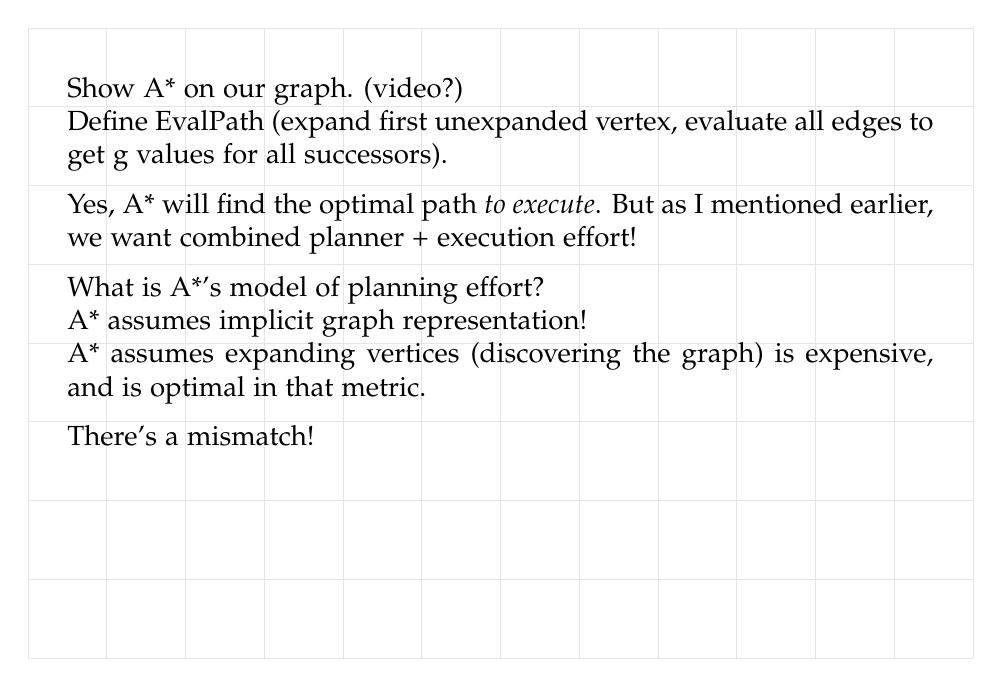
\begin{tikzpicture}
   
      \draw[step=1,black!10,very thin] (0,0) grid (12,8);
      
      \node[anchor=north] at (6,7.5)
      {
         \begin{minipage}[t]{11cm}
            Show A* on our graph. (video?)
            
            Define EvalPath (expand first unexpanded vertex,
            evaluate all edges to get g values for all successors).
            
            \medskip
            Yes, A* will find the optimal path \emph{to execute}.
            But as I mentioned earlier, we want combined planner + execution effort!
            
            \medskip
            What is A*'s model of planning effort?
            
            A* assumes implicit graph representation!
            
            A* assumes expanding vertices (discovering the graph)
            is expensive, and is optimal in that metric.
            
            \medskip
            There's a mismatch!
            
         \end{minipage}
      };
      
   \end{tikzpicture}
\end{frame}

\begin{frame}
   \frametitle{Explicit Graph Representation}
   
   Our graphs are small!
   
   Our EvalPath function can be different (e.g. bidirectional).
   Taken from RRTConnect.
   
   Maybe it will perform better?
   
   \begin{equation*}
      \hat{f}_x(\pi) = \sum_{e \in \pi} \left\{
      \begin{array}{cl}
         x[e] & \mbox{if edge } e \mbox{ evaluated}  \\
         \hat{x}(e) & \mbox{otherwise} \\
      \end{array}
      \right.
   \end{equation*}
   
   Similarity to front-to-front algorithms.
   
   This is how Lazy PRM works.
\end{frame}

\begin{frame}
   \frametitle{What about OUR planning effort estimate?}
   \begin{tikzpicture}
   
      \draw[step=1,black!10,very thin] (0,0) grid (12,8);
      
      \node[draw,line width=1.0pt,fill=blue!20,minimum width=0.75cm,minimum height=0.10cm]
         (Cfreebox) at (8.0, 7.5) {};
      \node[right=0cm of Cfreebox] {: $\mathcal{C}_{\mbox{\scriptsize free}}$}; 
      
      \node[inner sep=0] at (10.75,7) {%
         \includegraphics[width=2cm]{build/talk-act1-2d,graph}
      };
      
      % bfs
      %\only<1>{\fill[green!30] (0.5,5.6) rectangle (5.5,6.9);}
      %\only<2>{\fill[green!30] (0.5,5.6) rectangle (5.5,6.15);}
      %\only<3>{\fill[green!30] (0.5,6.15) rectangle (5.5,6.9);}
      \node at (2.5,6.75) {\begin{minipage}{5cm}
         \begin{algorithmic}
         \Loop%
            \State $\Pi \leftarrow $ \textsc{GetPaths}$()$
            \State $\pi^* \leftarrow \argmin\limits_{\pi \in \Pi} f(\pi)$
            \State \textsc{EvalPath}$(\pi^*)$
         \EndLoop
         \end{algorithmic}
         \end{minipage}
      };
      
      %\only<2>{
      %   \fill[green!30] (0.1,3.9) rectangle (5.9,4.9);
      %   \fill[green!30] (6.1,2.5) rectangle (11.9,4.9);
      %}
      \only<2>{
         \fill[green!30] (0.1,1.9) rectangle (5.9,2.8);
         \fill[green!30] (6.1,0.5) rectangle (11.9,1.6);
      }
      
      \node[inner sep=0pt,anchor=north] at (3,5.5) {
         \begin{minipage}[t]{5.5cm}%
            \hrule
            \vspace{0.1cm}
            Distance Model $\mathcal{M}_{\ms{dist}}$
            \begin{algorithmic}[1]
            \Function {$x_{\ms{\textup{dist}}}$}{$e$}
               \State \Return $|| q_e(1) - q_e(0) ||$
            \EndFunction
            \Function {$\hat{x}_{\ms{\textup{dist}}}$}{$e$}
               \State \Return $|| q_e(1) - q_e(0) ||$
            \EndFunction
            \only<2>{
               \Function {$\hat{p}_{\ms{\textup{dist}}}$}{$e$}
                  \State \Return $0$
               \EndFunction
            }
            \end{algorithmic}
            \hrule
         \end{minipage}%
      };
      
      \node[inner sep=0pt,anchor=north] at (9,5.5) {
         \begin{minipage}[t]{5.5cm}%
            \hrule
            \vspace{0.1cm}
            Set Validity Model $\mathcal{M}_{\ms{valid}}$
            \begin{algorithmic}[1]
            \Function {$x_{\ms{\textup{valid}}}$}{$e, \mathcal{C}_{\ms{free}}$}
               \If {${\bf 1}_{\ms{free}}[q_e(t)]$}
                  \State \Return $0$
               \Else
                  \State \Return $\infty$
               \EndIf
            \EndFunction
            \Function {$\hat{x}_{\ms{\textup{valid}}}$}{$e, \mathcal{C}_{\ms{free}}$}
               \State \Return $0$
            \EndFunction
            \only<2>{
               \Function {$\hat{p}_{\ms{\textup{valid}}}$}{$e, \mathcal{C}_{\ms{free}}$}
                  \State \Return $\hat{p}_{\ms{\textup{free}}}[q_e(t)]$
               \EndFunction
            }
            \end{algorithmic}
            \hrule
         \end{minipage}%
      };
      
   \end{tikzpicture}
\end{frame}

\begin{frame}
   \frametitle{Roadmaps $\rightarrow$ Graphs}
   \begin{tikzpicture}
   
      \draw[step=1,black!10,very thin] (0,0) grid (12,8);
      
      \node[inner sep=0] at (9,5) {%
         {\only<1-4>{\includegraphics{build/talk-act1-2d,graph}}}%
      };
      
      % legend
      \node[draw,line width=1.5pt,fill=blue!20,minimum width=0.75cm,minimum height=0.10cm]
         (Cfreebox) at (3.0, 7.0) {};
      \node[right=0cm of Cfreebox] {: $\mathcal{C}_{\mbox{\scriptsize free}}$}; 
      \node at (3,6.25) {$\Pi$ : set of candidate paths};
      
      \only<1-2>{\fill[green!30] (0.5,3.4) rectangle (5.5,4.1);}
      \only<3>{\fill[green!30] (0.5,2.9) rectangle (5.5,3.4);}
      \only<4>{\fill[green!30] (0.5,3.4) rectangle (5.5,4.1);}
      
      % bfs
      \node at (3,4) {\begin{minipage}{5cm}
         \begin{algorithmic}
         \Loop%
            \State $\Pi \leftarrow $ \textsc{GetPaths}$()$
            \State $\pi^* \leftarrow \argmin\limits_{\pi \in \Pi} f(\pi)$
            \State \textsc{EvalPath}$(\pi^*)$
         \EndLoop
         \end{algorithmic}
         \end{minipage}
      };
      
      \only<2-4>{%
         \node at (6,1) {\begin{minipage}{5cm}%
            \begin{equation*}%
            f(\pi) = {\hat f}_x(\pi) :
            \left\{ \begin{array}{ll}
                x(\pi) & \mbox{if } {\bf 1}_{\mbox{\scriptsize free}}(\pi) \\
                \infty & \mbox{otherwise}
            \end{array} \right.
         \end{equation*}
         \end{minipage}
         };
      }
      
   \end{tikzpicture}
\end{frame}





\begin{frame}
   \frametitle{Best-First Search over Paths: Graphs}
   \begin{center}
      \includegraphics{build/talk-act1-2d,graphfirstnext}
      
      \begin{minipage}{0.65\textwidth}
      \begin{algorithmic}
      \Loop
         \State $\Pi \leftarrow $ \textsc{GetPaths}$()$
            \Comment \tikz{\node[draw,circle,inner sep=0.7pt]{\scriptsize 1};}
         \State $\pi^* \leftarrow \argmin\limits_{\pi \in \Pi} f(\pi)$
            \Comment \tikz{\node[draw,circle,inner sep=0.7pt]{\scriptsize 2};}
         \State \textsc{EvalPath}$(\pi^*)$
            \Comment \tikz{\node[draw,circle,inner sep=0.7pt]{\scriptsize 3};}
      \EndLoop
      \end{algorithmic}
      \end{minipage}
      
      \begin{equation*}
         f_x(\pi) =
         \left\{ \begin{array}{ll}
             x(\pi) & \mbox{if } {\bf 1}_{\mbox{\scriptsize free}}(\pi) \\
             \infty & \mbox{otherwise}
         \end{array} \right.
      \end{equation*}
      
   \end{center}
\end{frame}

\begin{frame}
   \frametitle{Focus: Graph-based approaches}
   
   Let's search a graph in C-space.
   
   For now, assume a graph independent of Cfree,
   but we'll come back to this. (e.g. RRT, EST, PRM heuristics)
   
   (like basic PRM, lattice, FMT or BIT*-like thing)
   
   (talk just enough about C-space to give people an idea
   of the type of problem we're actually solving)
   
\end{frame}

\begin{frame}
   \frametitle{Graph formulation}
   
   Vertices are configurations (aka milestones).
   
   Edges are paths (e.g. local planner) and have a true cost.
   
   Start node and goal node.
   
   Traditional graph search objective: find lowest-cost path.
   
   Plot of execution vs planning effort.
   
   Talk about budgets and suboptimality guarantees?
   
   A*, Dijkstra's alg, Max's stuff?

\end{frame}

\begin{frame}
   \frametitle{Traditional problems}
   
   Huge graphs, so implicit representations.
   
   And so goal heuristics.
   
   Best-first search.
   
   Expanding vertices for successors is expensive (minimize expansions
   for time and space).
   
   Keeping open list sorted is expensive.
\end{frame}

\begin{frame}
   \frametitle{Our problem}
   
   Insight 1:
   But in our problem, graphs are SMALL,
   and edge evaluations are EXPENSIVE!
   
   Mention keyholes, we're not doing that!
   
   I call this an explicit graph with expensive edge evaluations.
   
   (Implicit representations are not necessary,
   and heuristics can be given the actual graph remaining.)
   
   This is one of the primary contribution of the PRM.
   
   Also talk about lazy PRM.
   
   Best-first over PATHS.
\end{frame}

\begin{frame}
   \frametitle{Planning effort objective}

   Relate to initial problem for motivation.

   Reference BUGSY algorithm (for implicit graphs).

   Introduce ensemble effort model.
   
   Show 2D example with radar.
\end{frame}

\begin{frame}
   \frametitle{Describe E8 algorithm.}
   
   Input: ensemble effort model.

   Talk about behaviour?
\end{frame}

\begin{frame}
   \frametitle{Simplification with proportional heuristics}

   Sidenote.

   Make equivalence claim to inflated search.
   
   Relate to E-graphs.
\end{frame}

\begin{frame}
   \frametitle{Return to continuous spaces.}

   Talk about E8 PRM.
   
   Independent of what kind of graph (lattice,
   progressively dense, etc).
   
   NAMED graphs that can be easily cached,
   removing nearest neighbor queries from the algorithm.
   
   Talk about parallelism?
   
   Show some results?
\end{frame}

\begin{frame}
   \frametitle{Sidenote: RRTs minimize planning effort only!}
   
   Should I talk about this?
\end{frame}

\begin{frame}
   \frametitle{How does this fail?}
   
   Talk about failure modes!
   
   This is a research question.
   
   Why optimistic?
   
   Behaviour.  Over-committing.  Similar to inflated heuristics.
   Behavior: over-commit, add in expectation?
\end{frame}

\begin{frame}
   \frametitle{Act 2: Planning with C-Space Families}
   
   Zoom out, we talked about each step,
   now lets talk about BETWEEN steps.
   
   We would like to reuse things!
\end{frame}

\begin{frame}
   \frametitle{Multi-object manipulation structure}
   
   Talk about full joint configuration space.
   
   In the simplest case with prehensile grasping,
   objects only move when the robot moves.
   
   When we project the joint C-space on the robot's dofs,
   each step of the plan manifests itself as a different Cfree.
   
   This motivates the study of planning with families of C-space subsets.
\end{frame}

\begin{frame}
   \frametitle{Example}
   
   Example of a multi-set situation.
   
   Forklift example?
   
   \includegraphics{build/figstar-a}
   
\end{frame}

\begin{frame}
   \frametitle{Subset Relations}
   
   Each subset has an indicator function.
   
   Insight 2:
   These subsets are related!
   
   Inclusions, intersections.
\end{frame}

\begin{frame}
   \frametitle{Example families}
   
   Start listing examples in manipulation.
   
   Cite lots of prior work!
   
   Caching, etc.

\end{frame}

\begin{frame}
   \frametitle{Multi-Set Formulation}
   
   Formulation!
\end{frame}

\begin{frame}
   \frametitle{Multi-Set PRM}
   
   Use PROPOSITIONAL LOGIC to represent subset relations
   as part of the ensemble effort model.
   
   Block diagram, with E8 PRM and 
\end{frame}

\begin{frame}
   \frametitle{How does this fail?}
   
   Talk about failure modes!
   
   This is a research question.
\end{frame}

\begin{frame}
   \frametitle{Act 3: Geometric task planning}
   
   Zoom out.
   
   How do we plan all these pieces for the COUPLED set of steps
   that does the task?
   
   Talk about the problem of any-to-any for the steps.
   
\end{frame}

\begin{frame}
   \frametitle{Blah blah CMR}
   
   What the heck do I talk about here.
   
   Baseline: commit early (e.g. from DRC paper, or HPN?).
   
\end{frame}

\begin{frame}
   \frametitle{Geometric Task planner proposed work}
   
   Insight 3: ??
   
   Talk about proposed work for geometric task planner.
   
\end{frame}

\begin{frame}
   \frametitle{Summary of Research Questions and Evaluations}
   
   summary of research questions.
   
\end{frame}

\begin{frame}
   \frametitle{Contributions}
   
   index of contributions.
   
   open-source software.
   
\end{frame}

\begin{frame}
   \frametitle{Timeline}
   
   Here is a timeline.
   
\end{frame}

\begin{frame}
   \frametitle{Last slide.}
   
   Summary from title.
   
   Brag about how awesome I am.
   
\end{frame}

\begin{frame}
   \frametitle{Best-First Search over Paths: Trajectory Optimization}
   \begin{center}
      \includegraphics{build/talk-act1-2d,traja}
      
      \begin{minipage}{0.65\textwidth}
      \begin{algorithmic}
      \Loop
         \State $\Pi \leftarrow $ \textsc{GetPaths}$()$
            \Comment \tikz{\node[draw,circle,inner sep=0.7pt]{\scriptsize 1};}
         \State $\pi^* \leftarrow \argmin\limits_{\pi \in \Pi} f(\pi)$
            \Comment \tikz{\node[draw,circle,inner sep=0.7pt]{\scriptsize 2};}
         \State \textsc{EvalPath}$(\pi^*)$
            \Comment \tikz{\node[draw,circle,inner sep=0.7pt]{\scriptsize 3};}
      \EndLoop
      \end{algorithmic}
      \end{minipage}
   \end{center}
\end{frame}

\begin{frame}
   \frametitle{Best-First Search over Paths: Trajectory Optimization}
   \begin{center}
      \includegraphics{build/talk-act1-2d,trajb}
      
      \begin{minipage}{0.8\textwidth}
      \begin{algorithmic}
      \Loop
         \State $\Pi \leftarrow $ \textsc{GetPaths}$()$
            \Comment Local neighborhood
         \State $\pi^* \leftarrow \argmin\limits_{\pi \in \Pi} f(\pi)$
            \Comment \tikz{\node[draw,circle,inner sep=0.7pt]{\scriptsize 2};}
         \State \textsc{EvalPath}$(\pi^*)$
            \Comment \tikz{\node[draw,circle,inner sep=0.7pt]{\scriptsize 3};}
      \EndLoop
      \end{algorithmic}
      \end{minipage}
   \end{center}
\end{frame}

\begin{frame}
   \frametitle{Best-First Search over Paths: Trajectory Optimization}
   \begin{center}
      \includegraphics{build/talk-act1-2d,trajc}
      
      \begin{minipage}{0.8\textwidth}
      \begin{algorithmic}
      \Loop
         \State $\Pi \leftarrow $ \textsc{GetPaths}$()$
            \Comment Local neighborhood
         \State $\pi^* \leftarrow \argmin\limits_{\pi \in \Pi} f(\pi)$
            \Comment $f(\pi):$ fuzzy approx
         \State \textsc{EvalPath}$(\pi^*)$
            \Comment \tikz{\node[draw,circle,inner sep=0.7pt]{\scriptsize 3};}
      \EndLoop
      \end{algorithmic}
      \end{minipage}
   \end{center}
\end{frame}

\begin{frame}
   \frametitle{Best-First Search over Paths: Trajectory Optimization}
   \begin{center}
      \includegraphics{build/talk-act1-2d,trajd}
      
      \begin{minipage}{0.8\textwidth}
      \begin{algorithmic}
      \Loop
         \State $\Pi \leftarrow $ \textsc{GetPaths}$()$
            \Comment Local neighborhood
         \State $\pi^* \leftarrow \argmin\limits_{\pi \in \Pi} f(\pi)$
            \Comment $f(\pi):$ fuzzy approx
         \State \textsc{EvalPath}$(\pi^*)$
            \Comment Re-linearize
      \EndLoop
      \end{algorithmic}
      \end{minipage}
   \end{center}
\end{frame}

\end{document}
